% !TeX spellcheck = ru_RU
% !TEX root = vkr.tex

\section{Модели и методы определения кода Голланда по данным психометрических тестов}

В данном разделе описываются различные подходы к предсказанию кода Голланда на полных данных (без пропусков) и на данных с пропусками, требующими восстановления. В конце раздела приводится итоговая структура решения задачи по предсказанию кода Голланда.

\subsection{Определение кода Голланда на полных данных: регрессия, классификация, ранжирование}

Данные психометрических тестов представляют собой набор признаков, принимающих целочисленные значения. Пример данных психометрических тестов приведен в таблице~\ref{tab:input_test_data}. Определение кода Голланда представляет собой предсказание шести чисел, отражающих степень выраженности типов личности (кодов Голланда). В качестве альтернативы набору из шести чисел предсказанием кода может служить ответ как в виде однобуквенного значения, так и набора из трех букв, \enquote{верхней триады}~--- тройки наиболее выраженных кодов. В случае, если в таком наборе задан порядок, то речь может идти о предсказании рангов кодов (от менее выраженного к наиболее выраженному).

\begingroup
  \fontsize{7pt}{8pt}\selectfont
  \begin{table}[ht]
    \centering
    \caption{Пример данных психометрических тестов}
    \label{tab:input_test_data}
    \begin{tabular*}{\textwidth}{
      @{\extracolsep{\fill}} 
      >{\centering\arraybackslash}p{0.8cm}       |  % id
      *{3}{>{\centering\arraybackslash}p{1.1cm}}    % BF
      >{\centering\arraybackslash}p{0.3cm}          % ...
      *{2}{>{\centering\arraybackslash}p{1.2cm}} |  % LN
      *{6}{>{\centering\arraybackslash}p{0.9cm}}    % HL
    }
        \toprule
        \multirow{2}{*}{\textbf{id}}
        & \multicolumn{3}{c}{\textbf{Бол. пятёрка}}
        & \multirow{2}{*}{\textbf{\dots}}
        & \multicolumn{2}{c|}{\textbf{Леонгард}}
        & \multicolumn{6}{c}{\textbf{Голланд}} \\
        \cmidrule(lr){2-4} \cmidrule(lr){6-7} \cmidrule(lr){8-13}
        & BF1 & BF2 & BF3 
        & 
        & LN9 & LN10 
        & HL1 & HL2 & HL3 & HL4 & HL5 & HL6 \\
        \midrule
        1 & 39 & 66 & 33 & \dots &  3 & 12  &  8 &  8 &  6 &  8 &  1 & 11 \\
        2 & 45 & 46 & 73 & \dots & 12 &  6  &  3 &  7 &  7 &  8 & 10 &  7 \\
        3 & 34 & 41 & 56 & \dots & 18 & 12  & 10 & 10 &  3 & 11 &  7 &  1 \\
        4 & 49 & 47 & 50 & \dots & 15 & 24  &  6 &  4 &  8 &  6 &  7 & 11 \\
        5 & 48 & 42 & 53 & \dots & 12 &  6  &  6 &  7 &  8 &  7 & 10 &  4 \\
        \bottomrule
    \end{tabular*}
  \end{table}
\endgroup

Таким образом, задача определения кода Голланда по результатам психометрических тестов личности может быть сведена к следующим задачам:
\begin{enumerate}[label={\arabic*)}]
    \item регрессия со множественными выходами (набор чисел);
    \item классификация (набор кодов);
    \item ранжирование (упорядоченный набор кодов);
    \item ансамблевые модели (комбинация базовых моделей).
\end{enumerate}


\subsubsection{Регрессия}
\label{subsec:regr}

Предсказание сразу нескольких целевых числовых переменных представляет собой регрессию со множественными выходами (многоцелевая регрессия, \emph{multitarget}). Существует три основных подхода к решению данной задачи~\cite{Spyromitros, Bishop}:
\begin{itemize}
    \item Применение моделей, по умолчанию поддерживающих множественные выходы (линейная регрессия, метод k-ближайших соседей, нейронные сети).
    \item Независимые предсказания каждого из выходов (\emph{multioutput}).
    \item Предсказания выходов по цепочке: последний предсказанный выход становится частью признакового пространства для предсказания следующего выхода (\emph{regressor chain}, см. рисунок \ref{fig:multioutput_regr}).
\end{itemize}

\begin{figure}[ht]
    \centering
    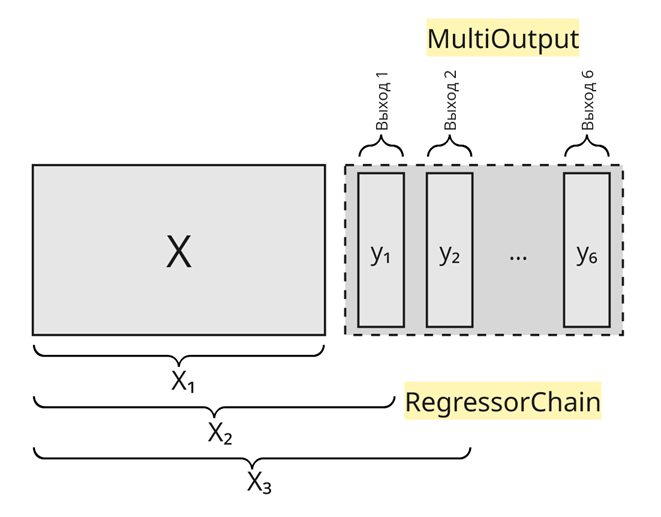
\includegraphics[width=0.75\linewidth]{figures/multioutput.png}
    \caption{Многоцелевая регрессия}
    \label{fig:multioutput_regr}
\end{figure}

Оцениваются результаты решения задачи регрессии со множественными выходами с помощью следующих усредненных по ответам метрик на тестовой выборке:
\begin{itemize}
    \item усредненная среднеквадратичная ошибка (RMSE);
    \item усредненный C-индекс (мера сходства, см. \ref{subsec:cindex}).
\end{itemize}

Лучшее качество обеспечивается при минимальных значениях RMSE и при максимальных значениях C-индекса (как мера согласованности). Чем больше С-индекс, тем большее сходство имеют два сравниваемых между собой профиля. Использование С-индекса позволяет сравнивать результаты не только с другими регрессионными задачами, но и, например, с задачами классификации. Стоит отметить, что в процессе обучения некоторые модели также позволяют оценить важность признаков: ансамблевые модели на основе решающих деревьев (случайный лес, градиентные бустинги) и линейные регрессоры.

Для нахождения взаимосвязей между факторами модели Голланда и другими психометрическими тестами в качестве базовых были использованы следующие регрессионные модели:
\begin{itemize}
    \item модели на основе линейной регрессии (простая линейная, пошаговая, L1-~и \mbox{L2-ре}\-гуля\-ризо\-ванные модели регрессии);
    \item модели на основе ансамблей деревьев с бутстрэппингом (случайный лес Random Forest, ExtraTrees);
    \item модели градиентного бустинга (XGBoost, LightGBM, CatBoost);
    \item непараметрические модели (kNN, SVR);
    \item нейросетевые модели (MLP, \emph{foundation-модель} TabPFN);
    \item базовая константная модель для сравнительного анализа.
\end{itemize}

При отсутствии пропусков (то есть при работе с \enquote{полными} данными) может быть целесообразным уменьшение размерности с помощью метода главных компонент (англ. \emph{Principal Component Analysis}, PCA)~\cite{Bishop}. Некоторые факторы различных тестов могут оценивать одни и те же аспекты личности, среди связей могут наблюдаться корреляции. Уменьшение размерности позволяет агрегировать схожие факторы тестов.


\subsubsection{Классификация}
\label{subsec:classif}

Предсказание одной или нескольких категориальных переменных (кодов, классов, меток) представляет собой задачу классификации. Предсказание кода Голланда как решение задачи классификации может быть сведено к следующим подходам~\cite{ZhangMin} (таблица~\ref{tab:class_types}):
\begin{itemize}
    \item Многоклассовая (\emph{multiclass}) классификация.\\
    Обучается один классификатор на шесть классов. В качестве ответа в порядке убывания вероятностей выбираются три наиболее вероятных кода.
    \item Многометочная (\emph{multilabel}) классификация.\\
    Обучаются шесть бинарных классификаторов, позволяющих дать ответ на вопрос, входит ли соответствующий код в \enquote{верхнюю триаду}. Выбираются три кода с наивысшими предсказанными вероятностями.
    \item Классификация на полное множество комбинаций (\emph{label powerset}).\\
    Всего существует 20 различных трехбуквенных комбинаций кода Голланда, в которых не учитывается порядок кодов. На выходе~--- тройка кодов. По причине отсутствия возможности учесть порядок кодов, для данного подхода невозможно использовать С-индекс, оценка которого основывается именно на порядке кодов.
\end{itemize}

\begingroup
\fontsize{7pt}{8pt}\selectfont
    \begin{table}[ht]
      \centering
      \caption{Подходы к классификации}
      \label{tab:class_types}
      \begin{tabular*}{0.95\textwidth}{@{\,}
        >{\centering\arraybackslash}m{3.8cm} |
        >{\centering\arraybackslash}m{4.2cm} |
        >{\centering\arraybackslash}m{4.5cm} |
        >{\centering\arraybackslash}m{2.5cm}}
        \toprule
        \textbf{Класси\-фикация}
          & \textbf{Модель}
          & \textbf{Значение}
          & \textbf{Пример} \\
        \midrule
        Много\-классовая (multiclass)
          & 1 классификатор на 6 классов
          & 3 однобуквенных кода
          & \texttt{R, S, E} \\
        \addlinespace[0.25em] \hline \addlinespace[0.25em]
        Много\-меточная (multilabel)
          & 6 бинарных классификаторов
          & Булевый вектор из 6 элементов с 3 значениями \texttt{True}
          & \texttt{[T, F, F, T, T, F]} \\
        \addlinespace[0.5em] \hline \addlinespace[0.25em]
        Множество комбинаций (label powerset)
          & 1 классификатор на 20 классов
          & трехбуквенный код, порядок кодов не важен
          & \texttt{RSE} \\
        \bottomrule
      \end{tabular*}
    \end{table}
\endgroup

По аналогии с решением задачи регрессии был применён метод главных компонент. Для оценки решения задачи классификации учитывалась метрика точности Top-K (\textit{Top-K accuracy}), которая показывает, в скольких случаях среди трех наиболее вероятных предсказанных моделью классов есть хотя бы \emph{K} правильно предсказанных меток. Например, $\text{Top-2}_{acc} = 0.7$ означает, что модель для 70\% предсказанных троек кодов угадала как минимум два истинных кода. Для сравнения с результатами других подходов также использовался \mbox{С-индекс}.

Для задачи классификации были взяты те же модели, что и для регрессии, за исключением нейросетевых моделей, а также с добавлением регуляризованных логистических регрессий (вместо линейных регрессий) и наивного байесовского классификатора.


\subsubsection{Ранжирование}
\label{subsec:ltr}

Представим задачу определения кода Голланда как задачу списочного ранжирования (\emph{listwise learn-to-rank})~\cite{Burges}. В отличие от поточечного ранжирования, где каждый элемент оценивается по шкале релевантности (что фактически сводится к задаче регрессии), или от попарного ранжирования, в котором моделируется относительный порядок пар элементов (бинарная классификация), списочное ранжирование рассматривает весь список результатов как единый упорядоченный объект.

Списочный подход требует задания двух ключевых компонентов: определения скоринговой функции и выбора функции потерь, оптимизирующей качество выдачи списка. В качестве скоринговой функции обычно используется многослойный перцептрон или более сложные архитектуры: глубокая перекрёстная сеть (\emph{Deep {\&} Cross Network}) либо трансформер с механизмом \emph{self‑attention}.

Типичными функциями потерь для списочного ранжирования являются NDCG (нормализованный дисконтированный совокупный прирост) и её дифференцируемые аппроксимации (ApproxNDCG, LambdaRank), а также специальные дифференцируемые функции, например ListNet, которая минимизирует кросс‑энтропию распределений релевантности и оптимизирует вероятность корректного попадания в топ‑k (в контексте решения задачи это топ‑1 и топ‑3).

Для оценки качества обученных моделей в качестве метрики часто используется \emph{NDCG@3}, отражающая \enquote{полезность} первых трёх элементов выдачи с учётом их позиций и релевантности; большее значение метрики качества \emph{NDCG@3} соответствует более точному ранжированию списков. В сравнении с другими видами ранжирования списочный подход обычно обеспечивает более высокую точность, однако требует значительных вычислительных ресурсов. В задачах с небольшим размером списка (шесть элементов) и ограниченным объёмом данных это ограничение, как правило, не является критическим.

Списочный подход демонстрирует высокую устойчивость к шуму в данных: оптимизация сразу всего списка способствует корректной расстановке элементов даже при неточных метках в обучении. Кроме того, такой подход дает возможность внедрения постоянного дообучения: по мере накопления новых оценок кодов Голланда модель можно дообучать на небольших батчах, сохраняя согласованность списков и не теряя ранее выученные связи между метками.


\subsubsection{Ансамблевые модели}
\label{subsec:ensemble}

Для улучшения качества прогноза можно использовать взвешенное ансамблирование моделей (линейный блендинг)~\cite{ZhangC}, когда итоговый ответ вычисляется как линейная комбинация предсказаний различных моделей с оптимизированными коэффициентами. Другим подходом является обучение метамодели на предсказаниях базовых моделей~--- стекинг.

Для стекинга были взяты следующие базовые модели:
\begin{itemize}[noitemsep, topsep=0pt, parsep=0pt, partopsep=0pt]
    \item линейные регрессии с различными параметрами регуляризации;
    \item L1- и L2-регуляризованные регрессии, LightGBM, CatBoost, случайный лес.
\end{itemize}
В обоих случаях метамоделью выступает обычная линейная регрессия. Важно отметить, что в первом случае при отсутствии регуляризации получалась бы линейная комбинация линейных моделей, что также является линейной моделью, и именно по этой причине добавляется нелинейная составляющая. Обучение базовых моделей происходит на обучающей выборке, обучение метамодели (подбор весов)~--- на валидационной, оценка метрик качества~--- на тестовой.

Для линейного блендинга (взвешенного ансамблирования) требуется найти, с каким весом будет входить в итоговое предсказание каждое из предсказаний базовых моделей. Таким образом, линейная комбинация весов моделей и их предсказания и будет итоговым предсказанием. Применяются следующие подходы для подбора весов~\cite{Bischl}:
\begin{description}
    \item[\textbullet] Равные веса всех моделей \\
    каждой базовой модели присваивается одинаковый вклад, что упрощает ансамблирование и служит базовой стратегией;
    \item[\textbullet] Вектор Шэпли~\cite{Sofiane}\\
    для каждого возможного порядка добавления моделей в ансамбль вычисляется разница в качестве при включении каждой модели в уже собранный набор, а затем усреднённые маргинальные приросты формируют распределение общего вклада каждого элемента ансамбля;
    \item[\textbullet] Частичный перебор по сетке\\
    поиск решений на предварительно заданной сетке возможных значений параметров (весов), при увеличении числа моделей для поиска вклада каждой предполагается использование подвыборки заданной сетки;
    \item[\textbullet] Квадратичная оптимизация (\emph{QP})\\
    решение задачи минимизации взвешенной суммы ошибок \mbox{ансамбля} как задачи квадратичного программирования с ограничениями;
    \item[\textbullet] Генетический алгоритм (\emph{GA})\\
    эволюционный поиск с выбором лучших представителей популяций (комбинаций весов), их скрещиванием и мутациями;
    \item[\textbullet] Метод роя частиц (\emph{PSO})~\cite{YouGui}\\
    оптимизация весов с помощью популяции частиц, которые перемещаются по пространству решений в соответствии с комбинацией собственного и глобального (популяции) оптимального пути;
    \item[\textbullet] Координатный спуск\\
    итеративная оптимизация веса каждой модели при фиксации остальных.
\end{description}
Стоит отметить, что лишь метод квадратичного программирования предполагает, что функция потерь является непрерывно дифференцируемой. Ансамблирование также служит естественным регуляризатором: при объединении слабых и сильных моделей, уменьшается риск переобучения отдельных компонентов, поскольку ошибки одних моделей компенсируются другими, что особенно ценно при ограниченном объёме данных.


\subsection{Математическое обеспечение модуля восстановления данных психометрических тестов}
\label{subsec:imput}

В исходной задаче предполагается наличие пропусков (неполноты) в данных, поскольку пользователь мог и не успеть пройти пять психометрических тестов перед тем, как запрашивается предсказание его кода Голланда. Игнорирование таких записей приведёт либо к значительному сужению выборки (при удалении неполных строк), либо к искажению итоговых оценок. Существуют следующие подходы для восстановления (импутации) данных отсутствующих тестов~\cite{Buuren}:

\begin{enumerate}[label={\arabic*)}]
    \item множественная импутация цепочными уравнениями (\emph{MICE});
    \item низкоранговая матричная аппроксимация (\emph{Matrix Soft Impute});
    \item применение масок для пропущенных значений;
    \item взвешенное ансамблирование комбинации заполненных тестов.
\end{enumerate}

Метод MICE (от англ. \emph{Multivariate Imputation by Chained Equations}) заключается в поочерёдном построении для каждого признака с пропусками регрессионной модели на основе остальных переменных; заполнение пропусков выполняется итеративно в несколько циклов до сходимости. При этом на каждом шаге для конкретного признака используются актуализированные значения остальных признаков, что позволяет учитывать их взаимные зависимости и уменьшать смещение оценок. После завершения всех итераций получается несколько \enquote{полных} наборов данных, что даёт возможность оценить неопределённость импутации и корректно скорректировать дисперсию итоговых показателей. Однако метод MICE для обработки \textit{каждой отдельной записи} требует наличия значений по всем остальным признакам: модель фактически \enquote{дообучается} на лету при каждом новом наблюдении. Кроме того, при сильной корреляции между переменными могут возникать нестабильность процесса итеративной импутации и проблемы со сходимостью алгоритма.

Метод \emph{Soft Impute} (мягкое матричное восстановление) строит низкоранговую аппроксимацию матрицы с пропусками через регуляризованное сингулярное разложение (SVD, \emph{Singular Value Decomposition}). На каждой итерации отсутствующие элементы заполняются текущими оценками, затем матрица подвергается сингулярному разложению на собственные значения и собственные векторы, после чего к собственным значениям применяется мягкое пороговое преобразование: все значения, не превышающие параметр $\lambda$, обнуляются, а остальные уменьшаются на величину $\lambda$. Повторяя эти шаги до сходимости, алгоритм одновременно минимизирует ошибку восстановления и контролирует ранжирование компонентов через ядерную норму. Подход, лежащий в основе \emph{Soft Impute}, обеспечивает масштабируемость за счёт применения приближённых алгоритмов сингулярного разложения (SVD).

Находит применение и использование бинарных индикаторов пропусков (масок)~--— это дополнительные признаки, принимающие значение \enquote{1} при отсутствии исходного измерения и \enquote{0} в противном случае. Данный приём не восстанавливает значения пропущенных факторов, а лишь информирует модель о факте выпадения данных, что позволяет учитывать механизмы образования пропусков и повышать устойчивость прогнозов при информативном пропуске. Включение масок пропусков способствует обнаружению зависимостей между фактом отсутствия и целевой переменной, однако повышает размерность признакового пространства и может усложнить обучение моделей за счёт роста числа параметров.

Взвешенное ансамблирование (блендинг) по комбинации тестов предполагает построение отдельного ансамбля для каждой из 31 возможной комбинации заполненных пользователем тестов. Для каждой комбинации подбираются веса базовых моделей с учётом только тех признаков, которые доступны в данном случае, что позволяет максимально адаптировать прогноз к фактическим данным. Такой подход позволяет учесть специфические взаимосвязи между тестами и улучшить точность в каждой группе пользователей, однако требует обучения и хранения 31 набора весов, что значительно увеличивает вычислительные затраты и объём памяти. Кроме того, при появлении новых сочетаний тестов необходимо обновлять все ансамбли, что усложняет сопровождение и масштабирование решения.

В зависимости от объёма и характера пропусков оптимальный выбор метода восстановления данных может различаться: при умеренном уровне неполноты и выраженных корреляциях между тестами MICE и низкоранговая матричная аппроксимация обеспечивают более точное восстановление, тогда как маски пропусков и ансамблирование по комбинациям позволяют обойтись без генерации синтетических значений и сохраняют прозрачность модели. В вычислительном плане методы матричной аппроксимации и применения масок пропусков предпочтительны: оба подхода масштабируются за счёт простой векторизированной реализации и минимально увеличивают объём параметров.


\subsection{Итоговая структура решения задачи по определению кода Голланда}

Решение задачи по предсказанию кода Голланда предполагает нахождение лучших вариантов на каждом из следующих этапов экспериментального исследования:
\begin{enumerate}[noitemsep, topsep=2pt, parsep=0pt, partopsep=0pt]
    \item Восстановление данных тестов, которые не были заполнены.
    \item Уменьшение размерности входных данных.
    \item Тип решения задачи.
    \item Подход в зависимости от типа решения задачи.
    \item Базовые модели для каждого из подходов.
    \item Настройка гиперпараметров моделей.
    \item Взвешенное ансамблирование базовых моделей.
\end{enumerate}

\begin{figure}[htb]
    \centering
    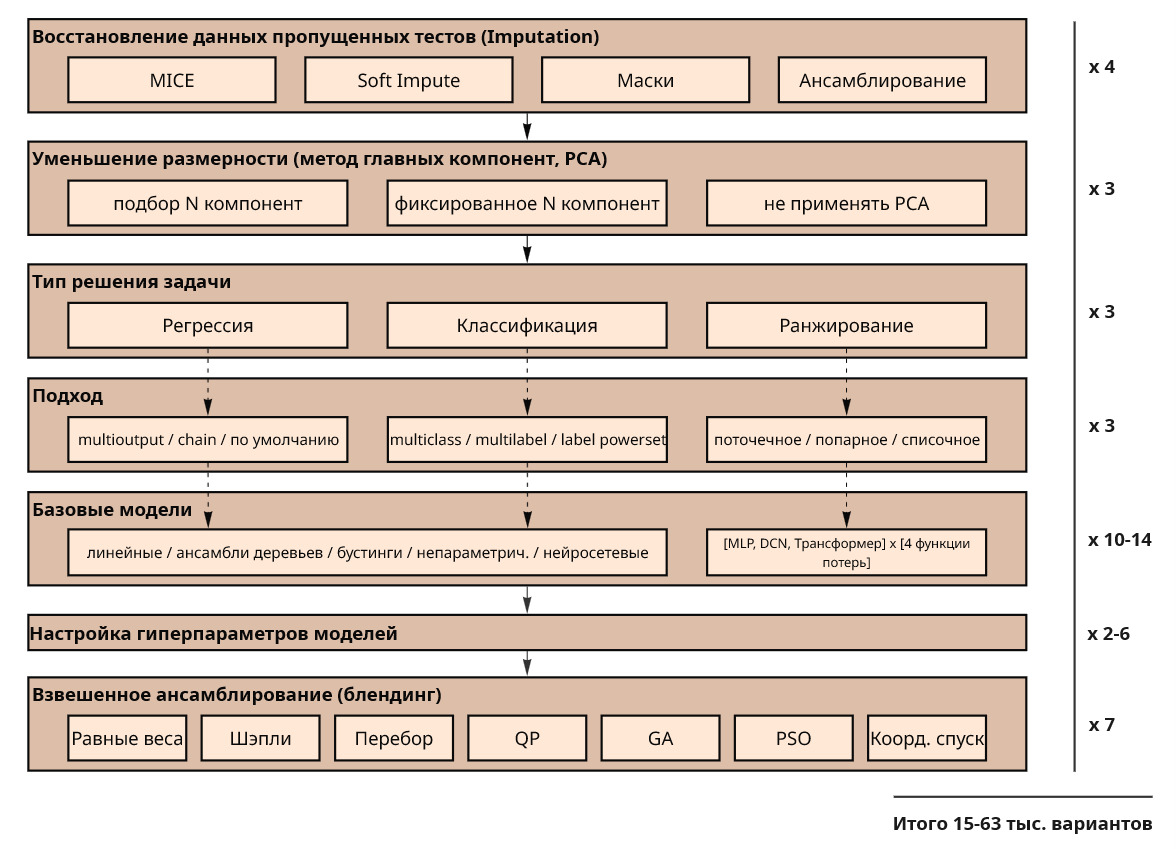
\includegraphics[width=1\linewidth]{figures/multi_pipeline.jpg}
    \caption{Общая схема вариантов экспериментального исследования}
    \label{fig:multi_pipeline}
\end{figure}

Общая схема вариантов экспериментального исследования представлена на  рисунке~\ref{fig:multi_pipeline}. Оценка каждого варианта проводится в соответствии с мерой сходства C-индекс. 

Следует отметить, что этап уменьшения размерности может:
\begin{itemize}[noitemsep, topsep=0pt, parsep=0pt, partopsep=0pt]
    \item[-] не выполняться вовсе;
    \item[-] применяться с фиксированным порогом на уровне 90\% объяснённой дисперсии;
    \item[-] выполняться с динамическим подбором числа компонент (N).
\end{itemize}
На этапе ранжирования поточечный и попарный подходы могут пропускаться в пользу списочного (\emph{listwise}). Конкретный выбор базовых моделей регрессии и классификации более подробно описан в разделах~\ref{subsec:regr} и~\ref{subsec:classif}. Для списочного ранжирования рассматриваются все возможные комбинации трёх архитектур (многослойный перцептрон, глубокая перекрёстная сеть, трансформер) и четырёх функций потерь (\textsc{ApproxNDCG}, \textsc{ListNet@1}, \textsc{ListNet@3}, \textsc{LambdaRank}). Каждая из базовых моделей также требует подбора гиперпараметров, например, числа ближайших соседей \textit{k} для модели kNN. Итоговое число вариантов для перебора и определения наилучшего способа предсказания кода Голланда может достигать 63 тысяч различных способов, что создаёт значительную вычислительную нагрузку.
